\chapter{Code validation}
\section{Single phase validation}
The code was validated running a simulation at $\Re_\tau=300$ starting from a fully developed turbulent channel flow; all the results were gathered on a timespan of 1\,500 $t^+$. The results were then compared with the DNS database of \cite{thtlab} at the same shear Reynolds number. Here is presented the outcome of this comparison; the data from \cite{thtlab} are denoted as tht-lab in the following pictures.\\
The velocity skewness was also compared with the old code results (\texttt{FlOWSB}), showing a perfect agreement.
\begin{figure}[H]
\centering
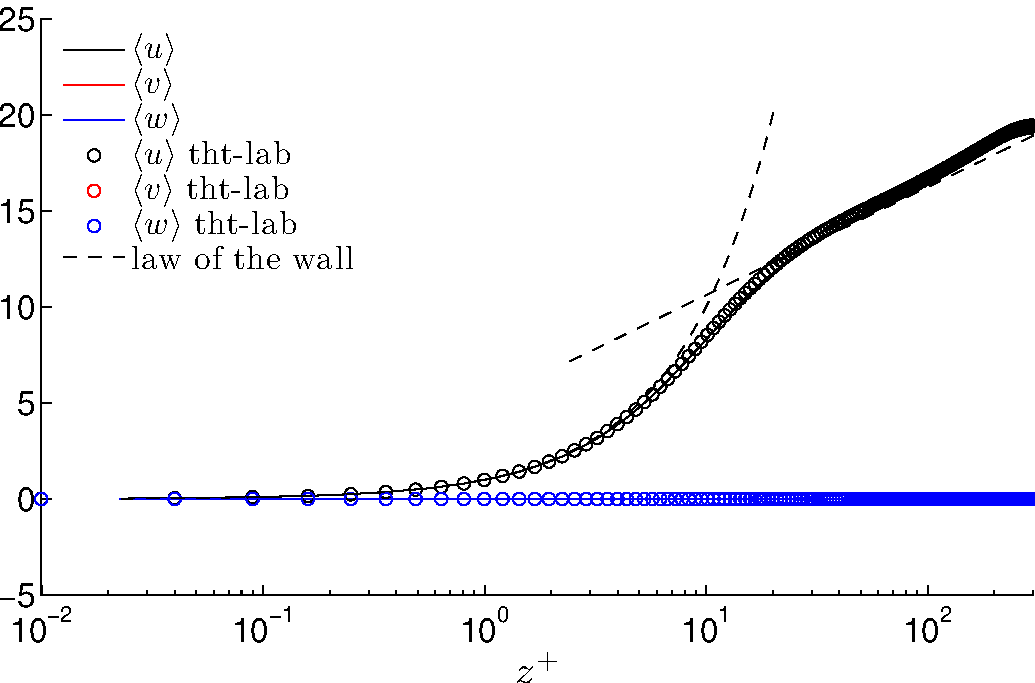
\includegraphics[width=\textwidth]{mean}
\caption{Mean velocity}
\end{figure}
\begin{figure}[H]
\centering
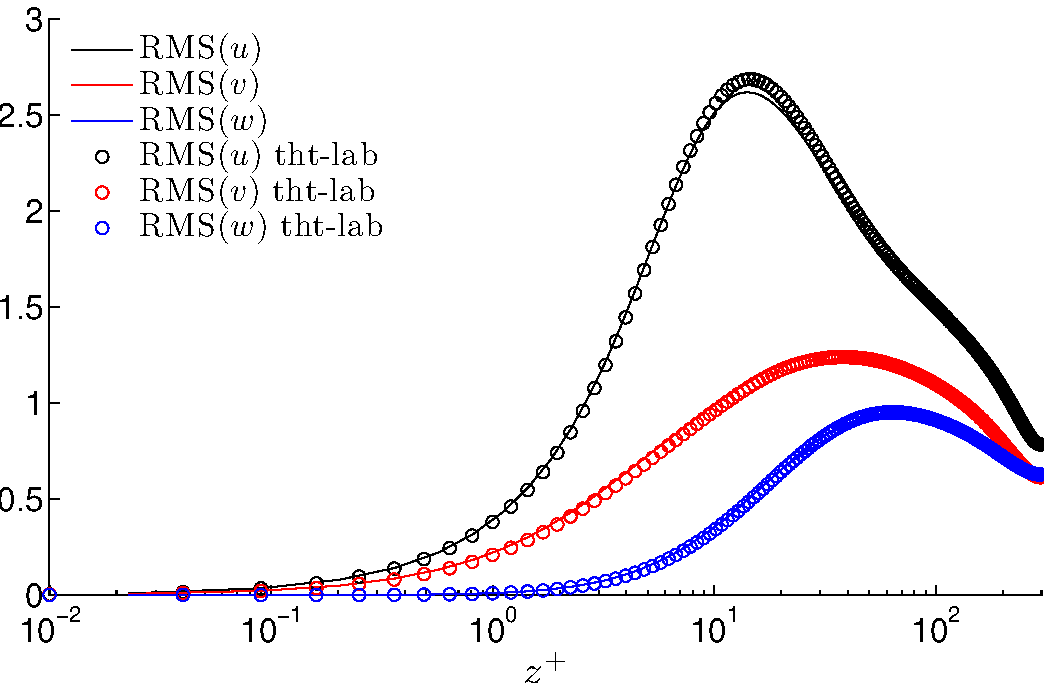
\includegraphics[width=\textwidth]{rms}
\caption{Velocity root mean square}
\end{figure}
\begin{figure}[H]
\centering
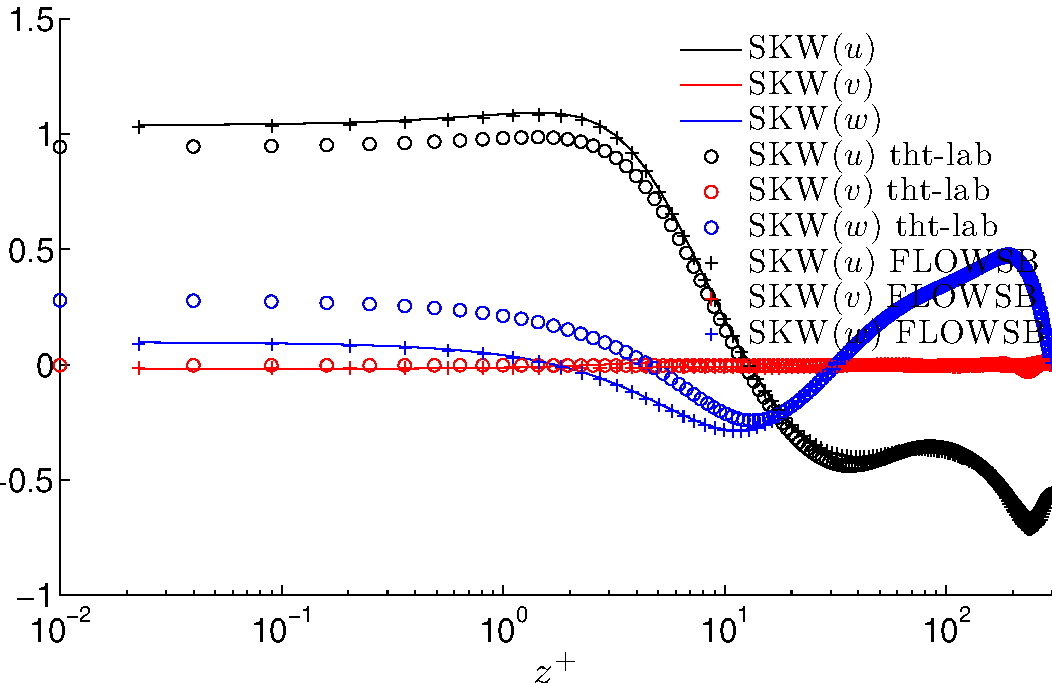
\includegraphics[width=\textwidth]{skw}
\caption{Velocity skewness}
\end{figure}
\begin{figure}[H]
\centering
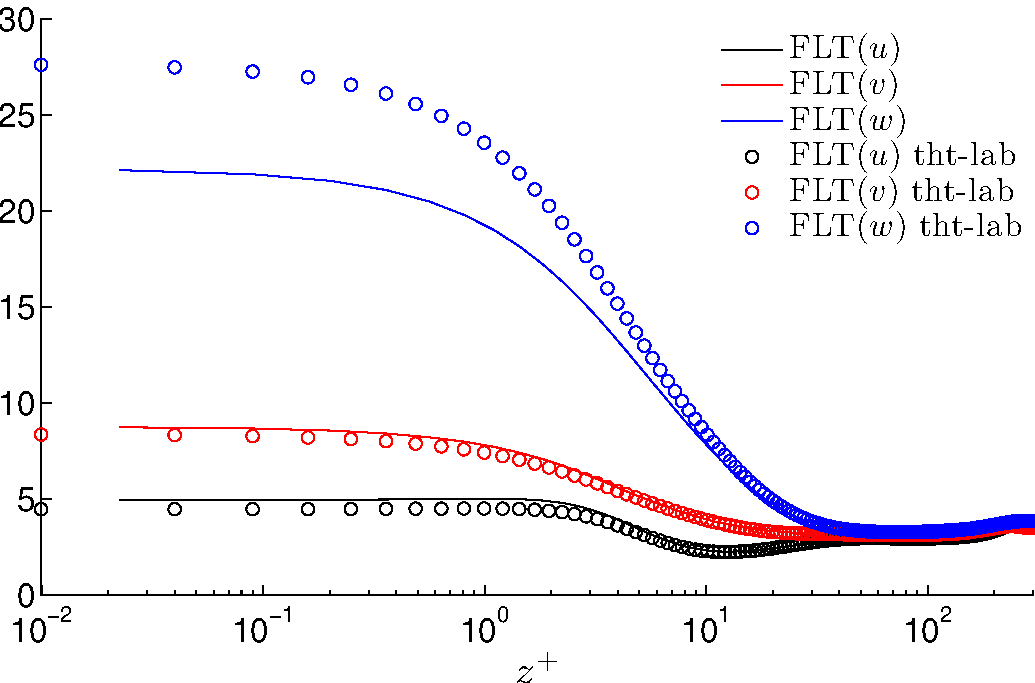
\includegraphics[width=\textwidth]{flt}
\caption{Velocity flatness}
\end{figure}
\begin{figure}[H]
\centering
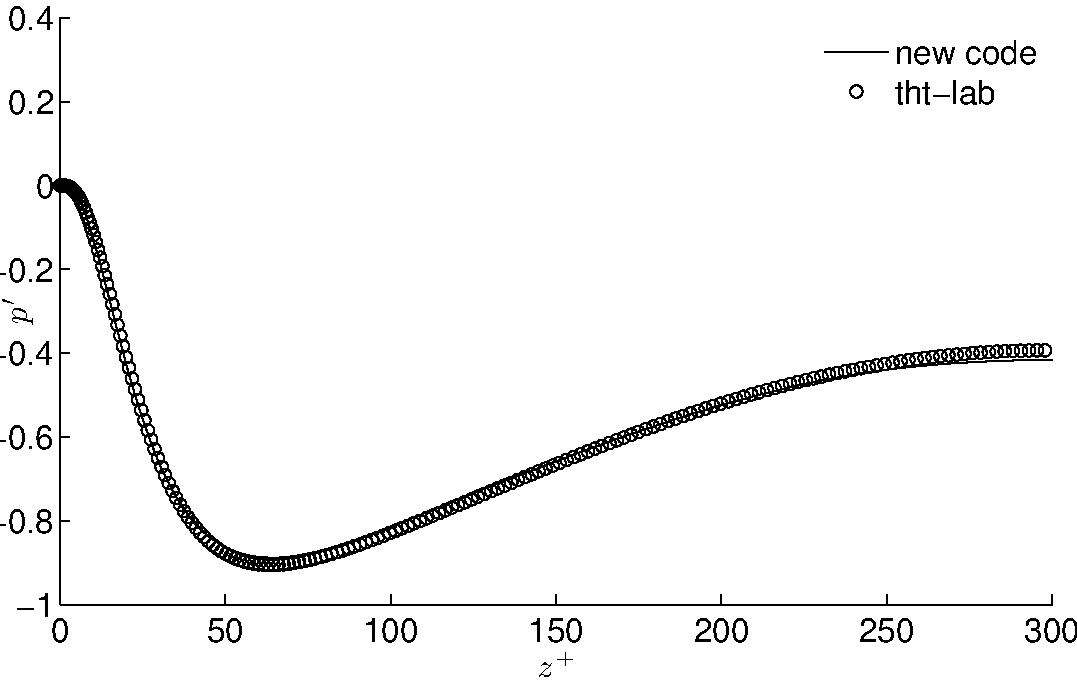
\includegraphics[width=\textwidth]{pmean}
\caption{Mean pressure}
\end{figure}
\begin{figure}[H]
\centering
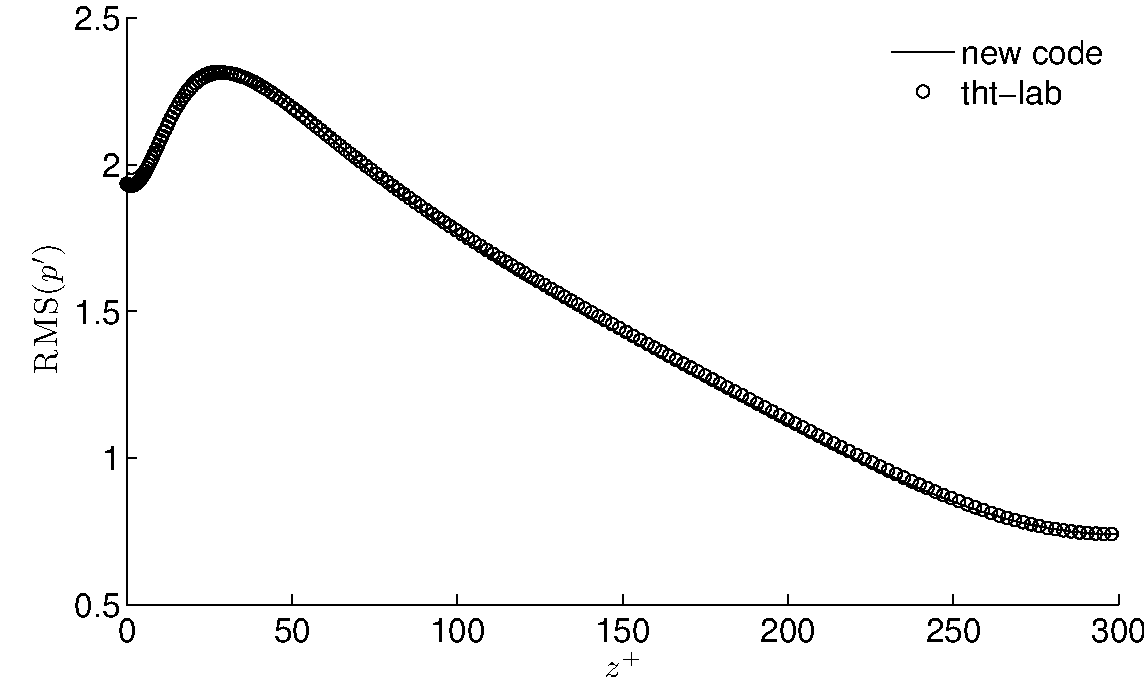
\includegraphics[width=\textwidth]{prms}
\caption{Pressure root mean square}
\end{figure}
\begin{sidewaysfigure}
\centering
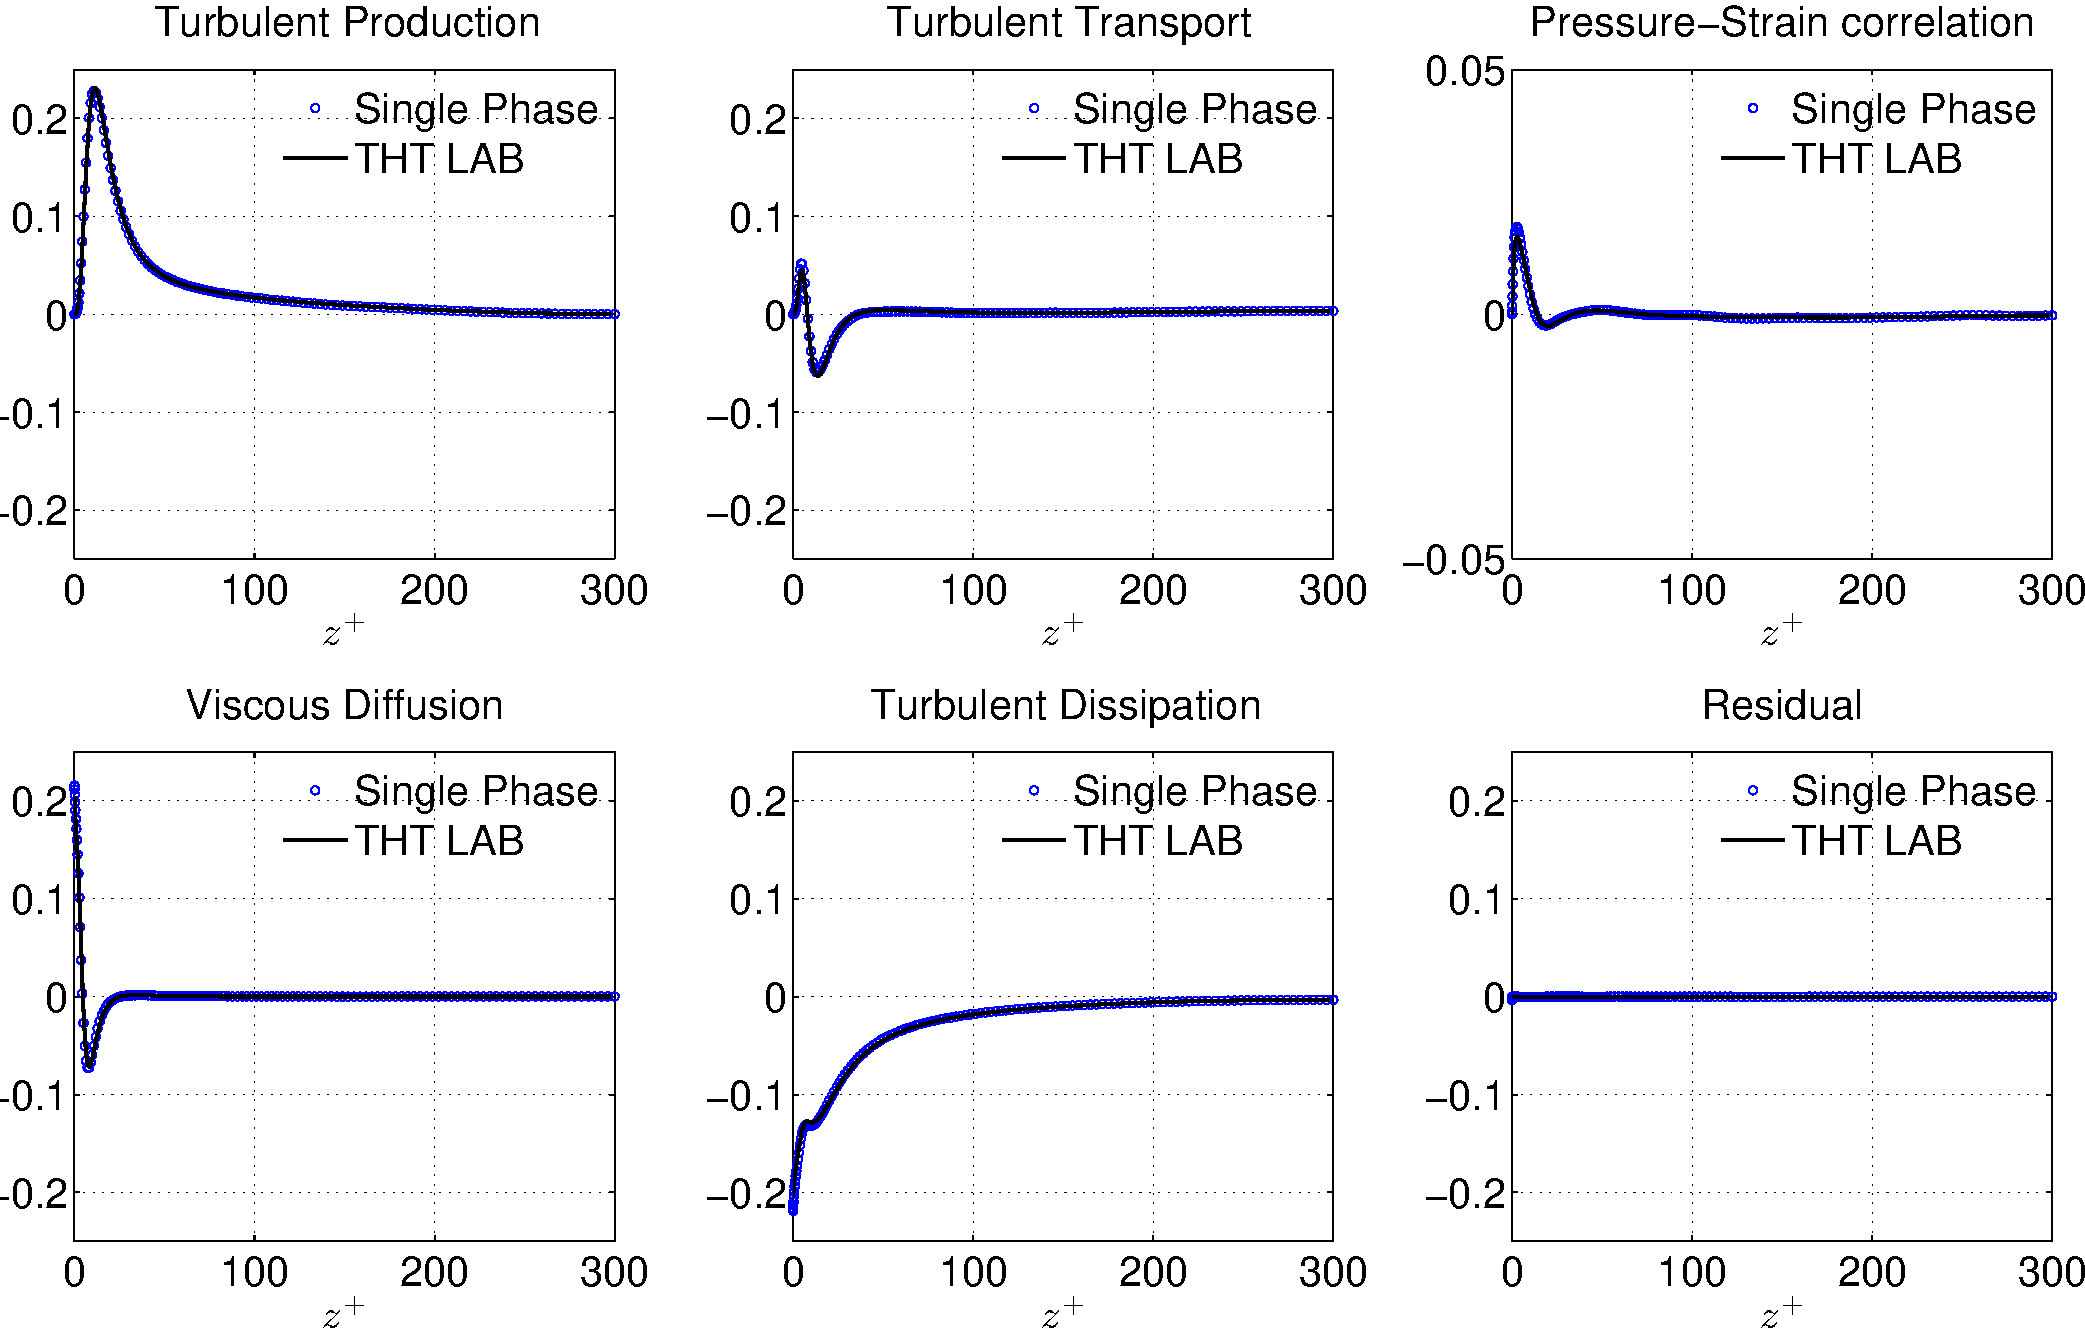
\includegraphics[width=\textwidth]{budget}
\caption{Energy budget}
\end{sidewaysfigure}
\begin{sidewaysfigure}
\centering
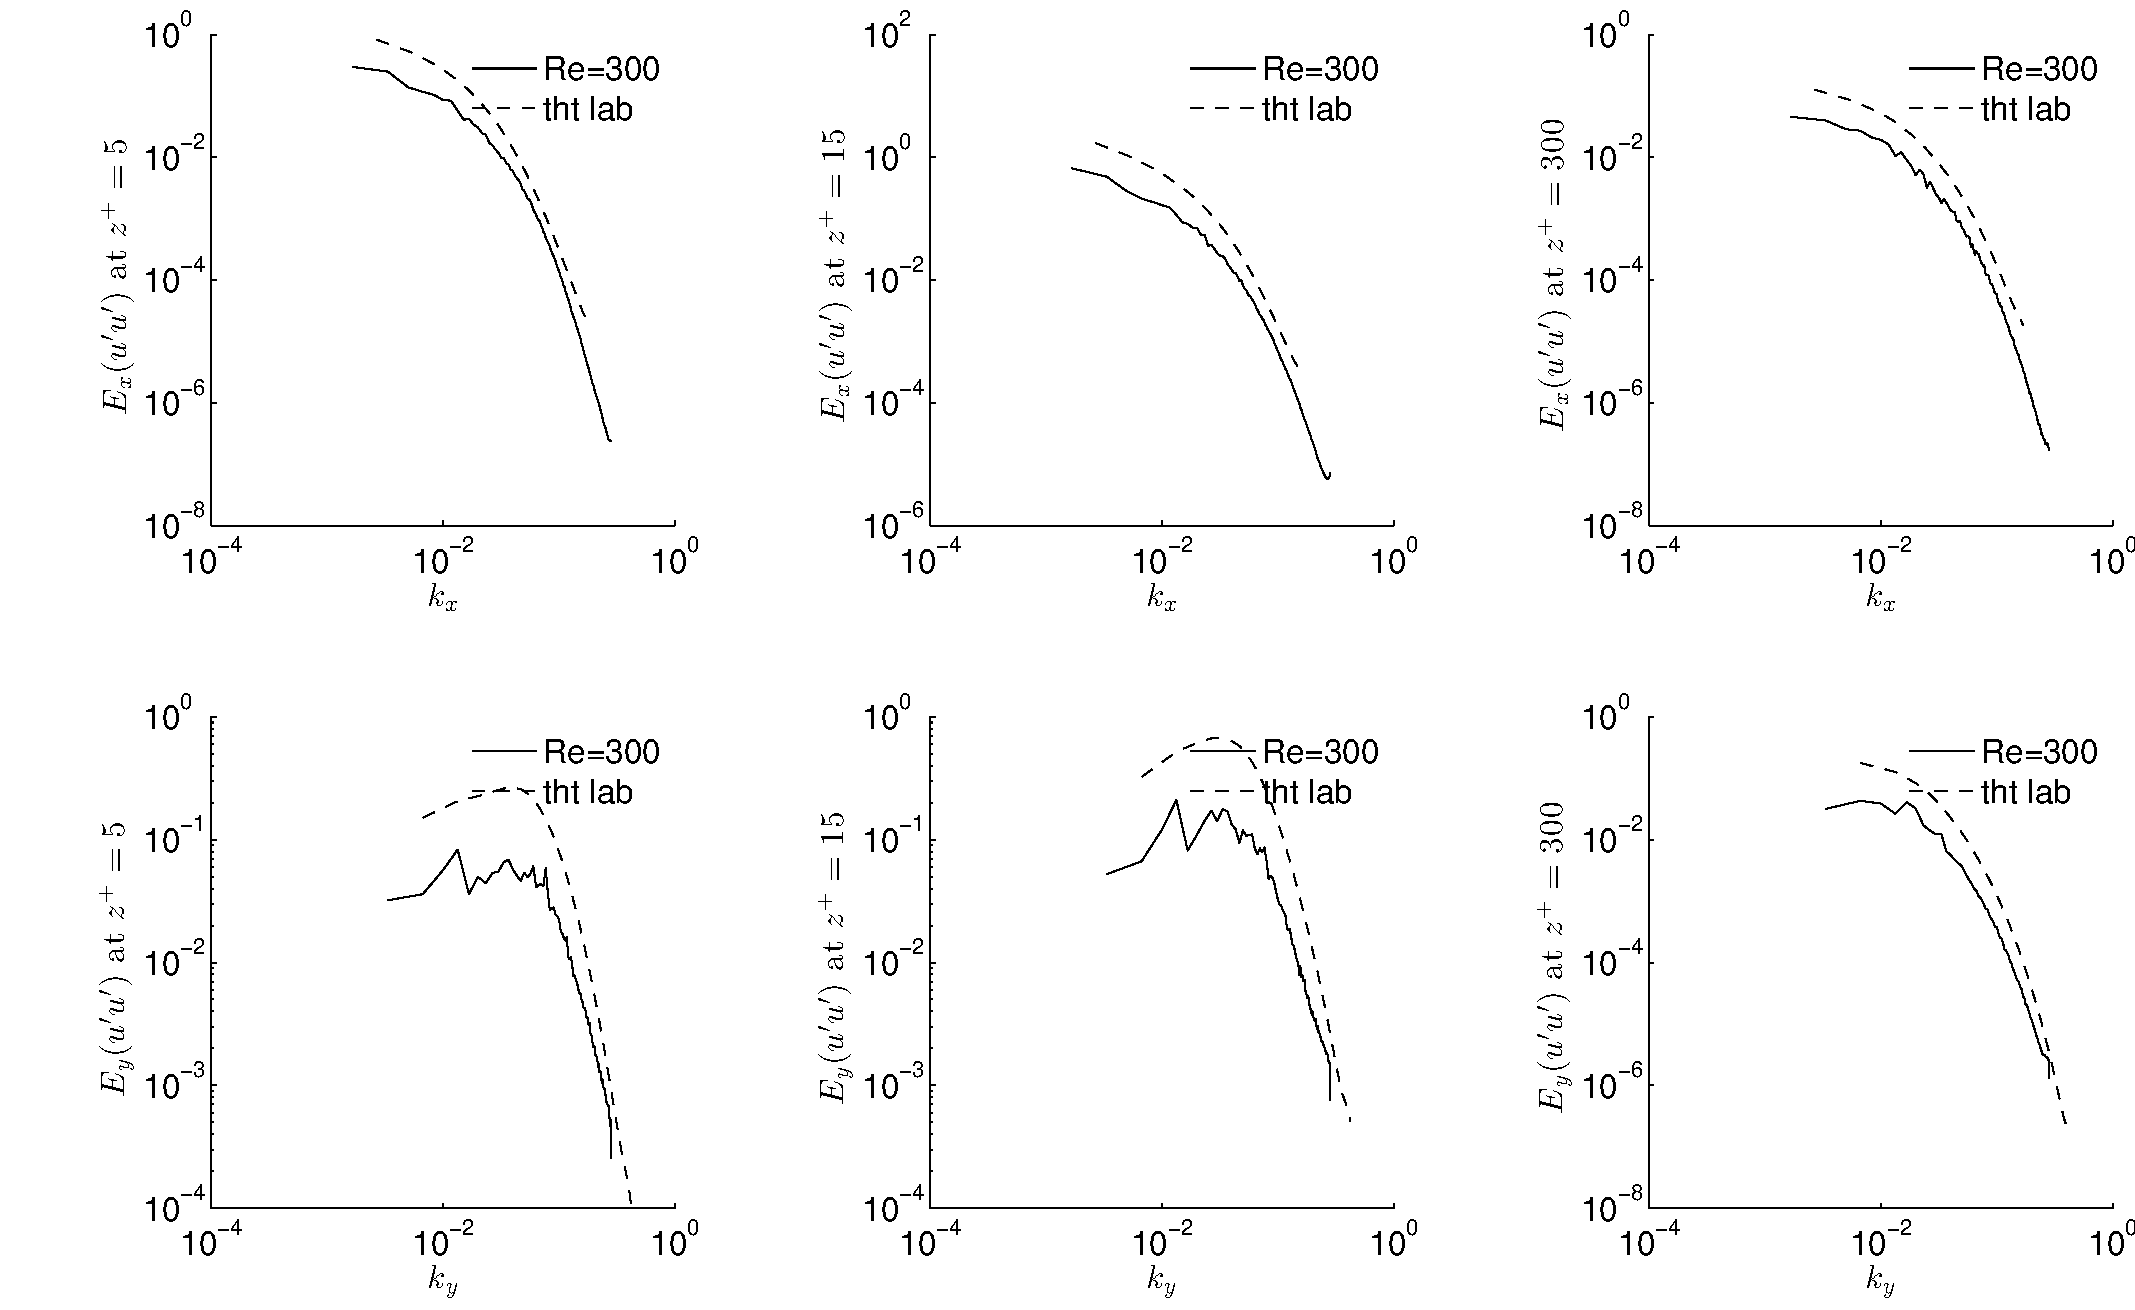
\includegraphics[width=\textwidth]{u_spectra}
\caption{$u'$ power spectra}
\end{sidewaysfigure}
\begin{sidewaysfigure}
\centering
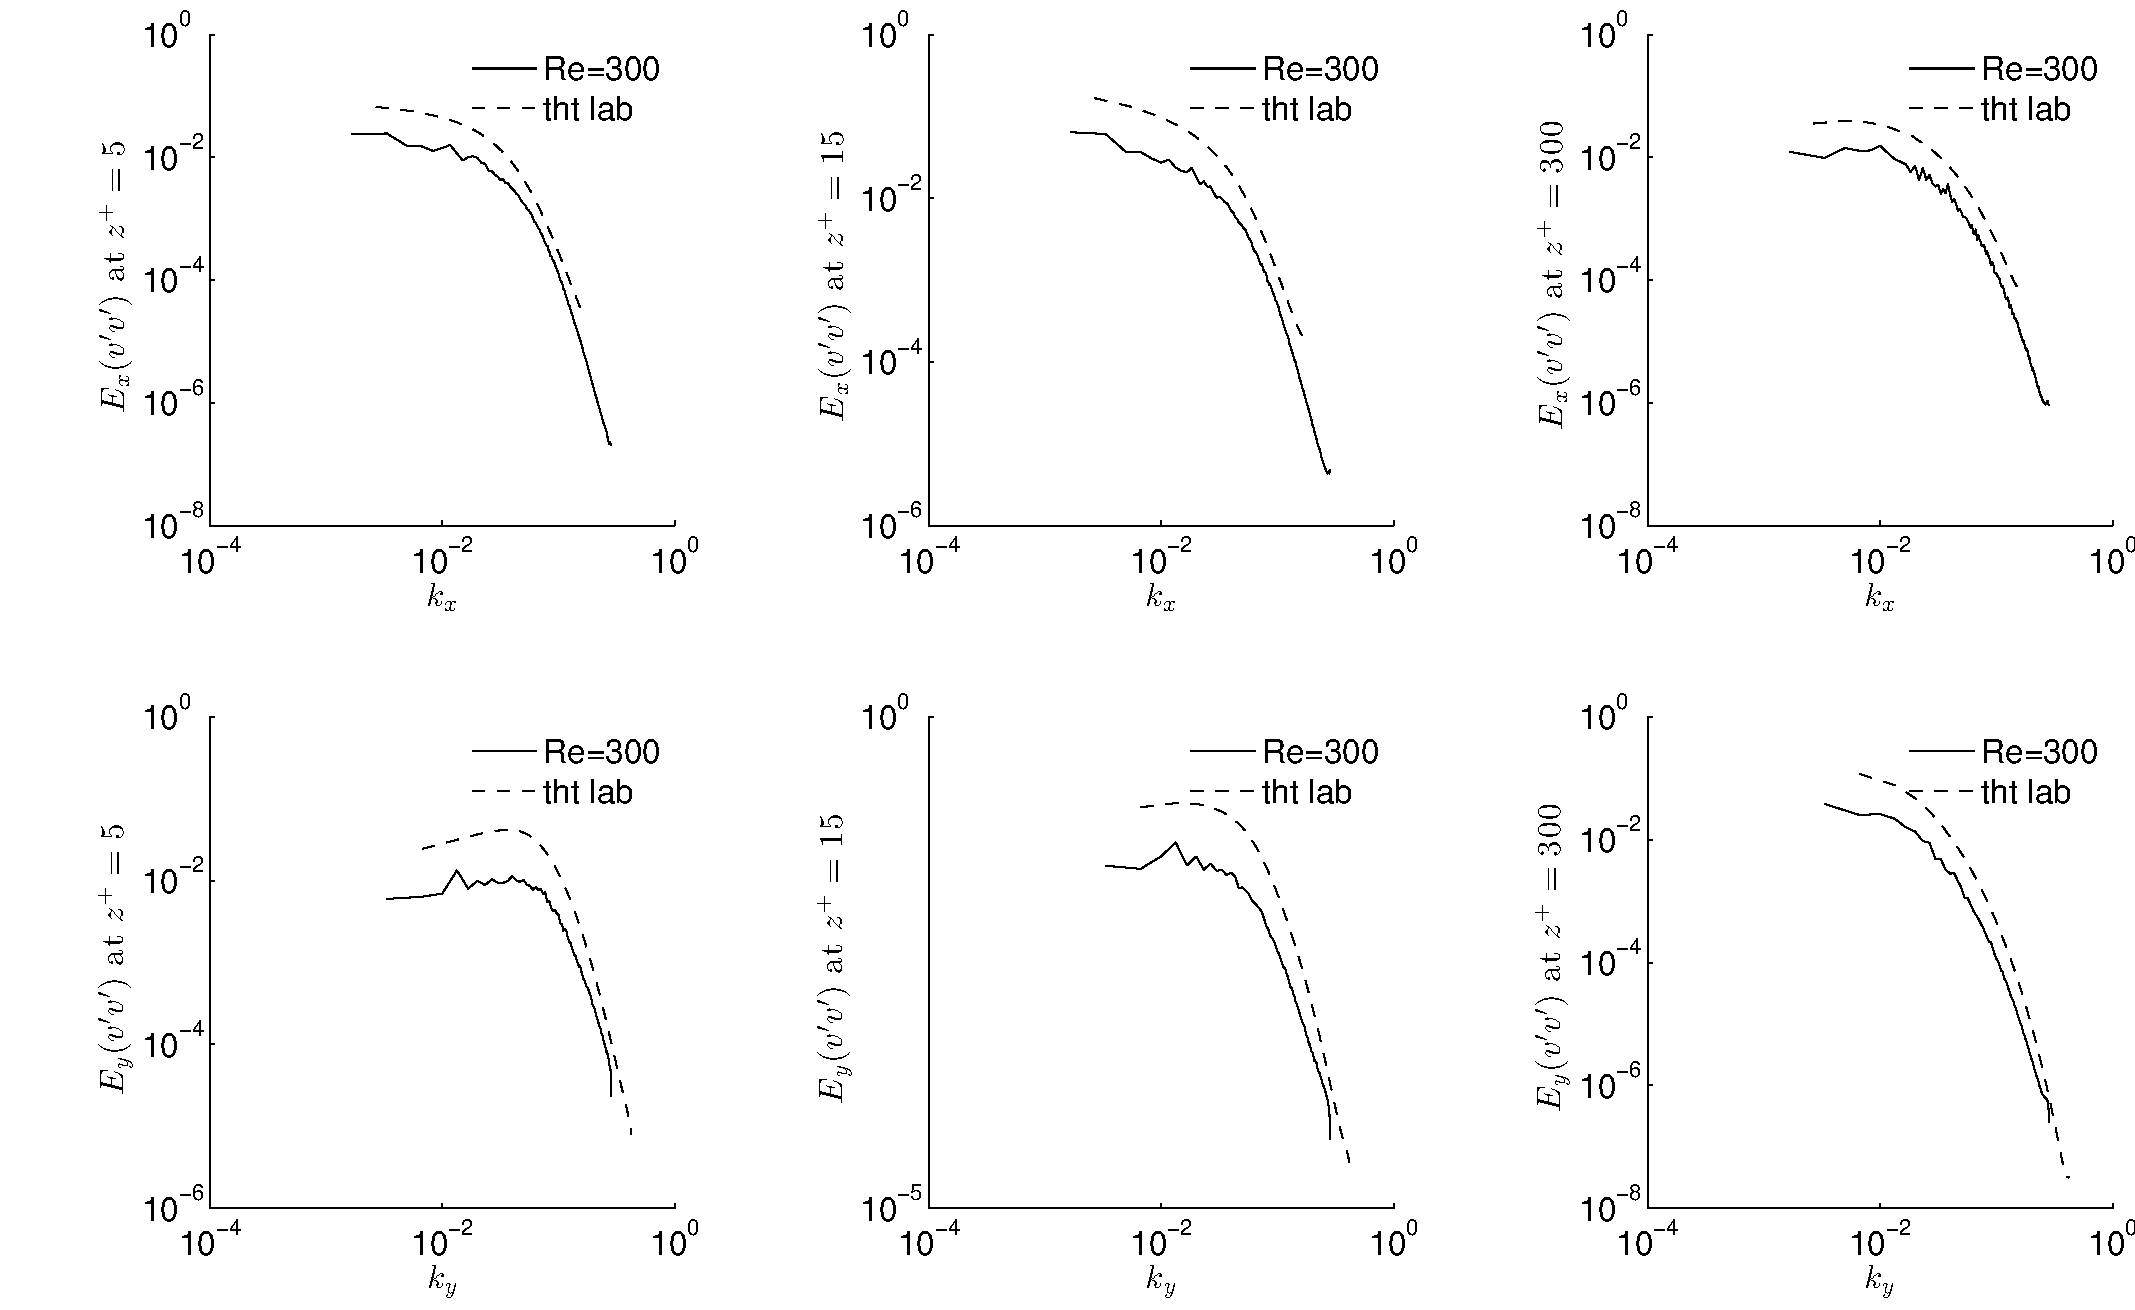
\includegraphics[width=\textwidth]{v_spectra}
\caption{$v'$ power spectra}
\end{sidewaysfigure}
\begin{sidewaysfigure}
\centering
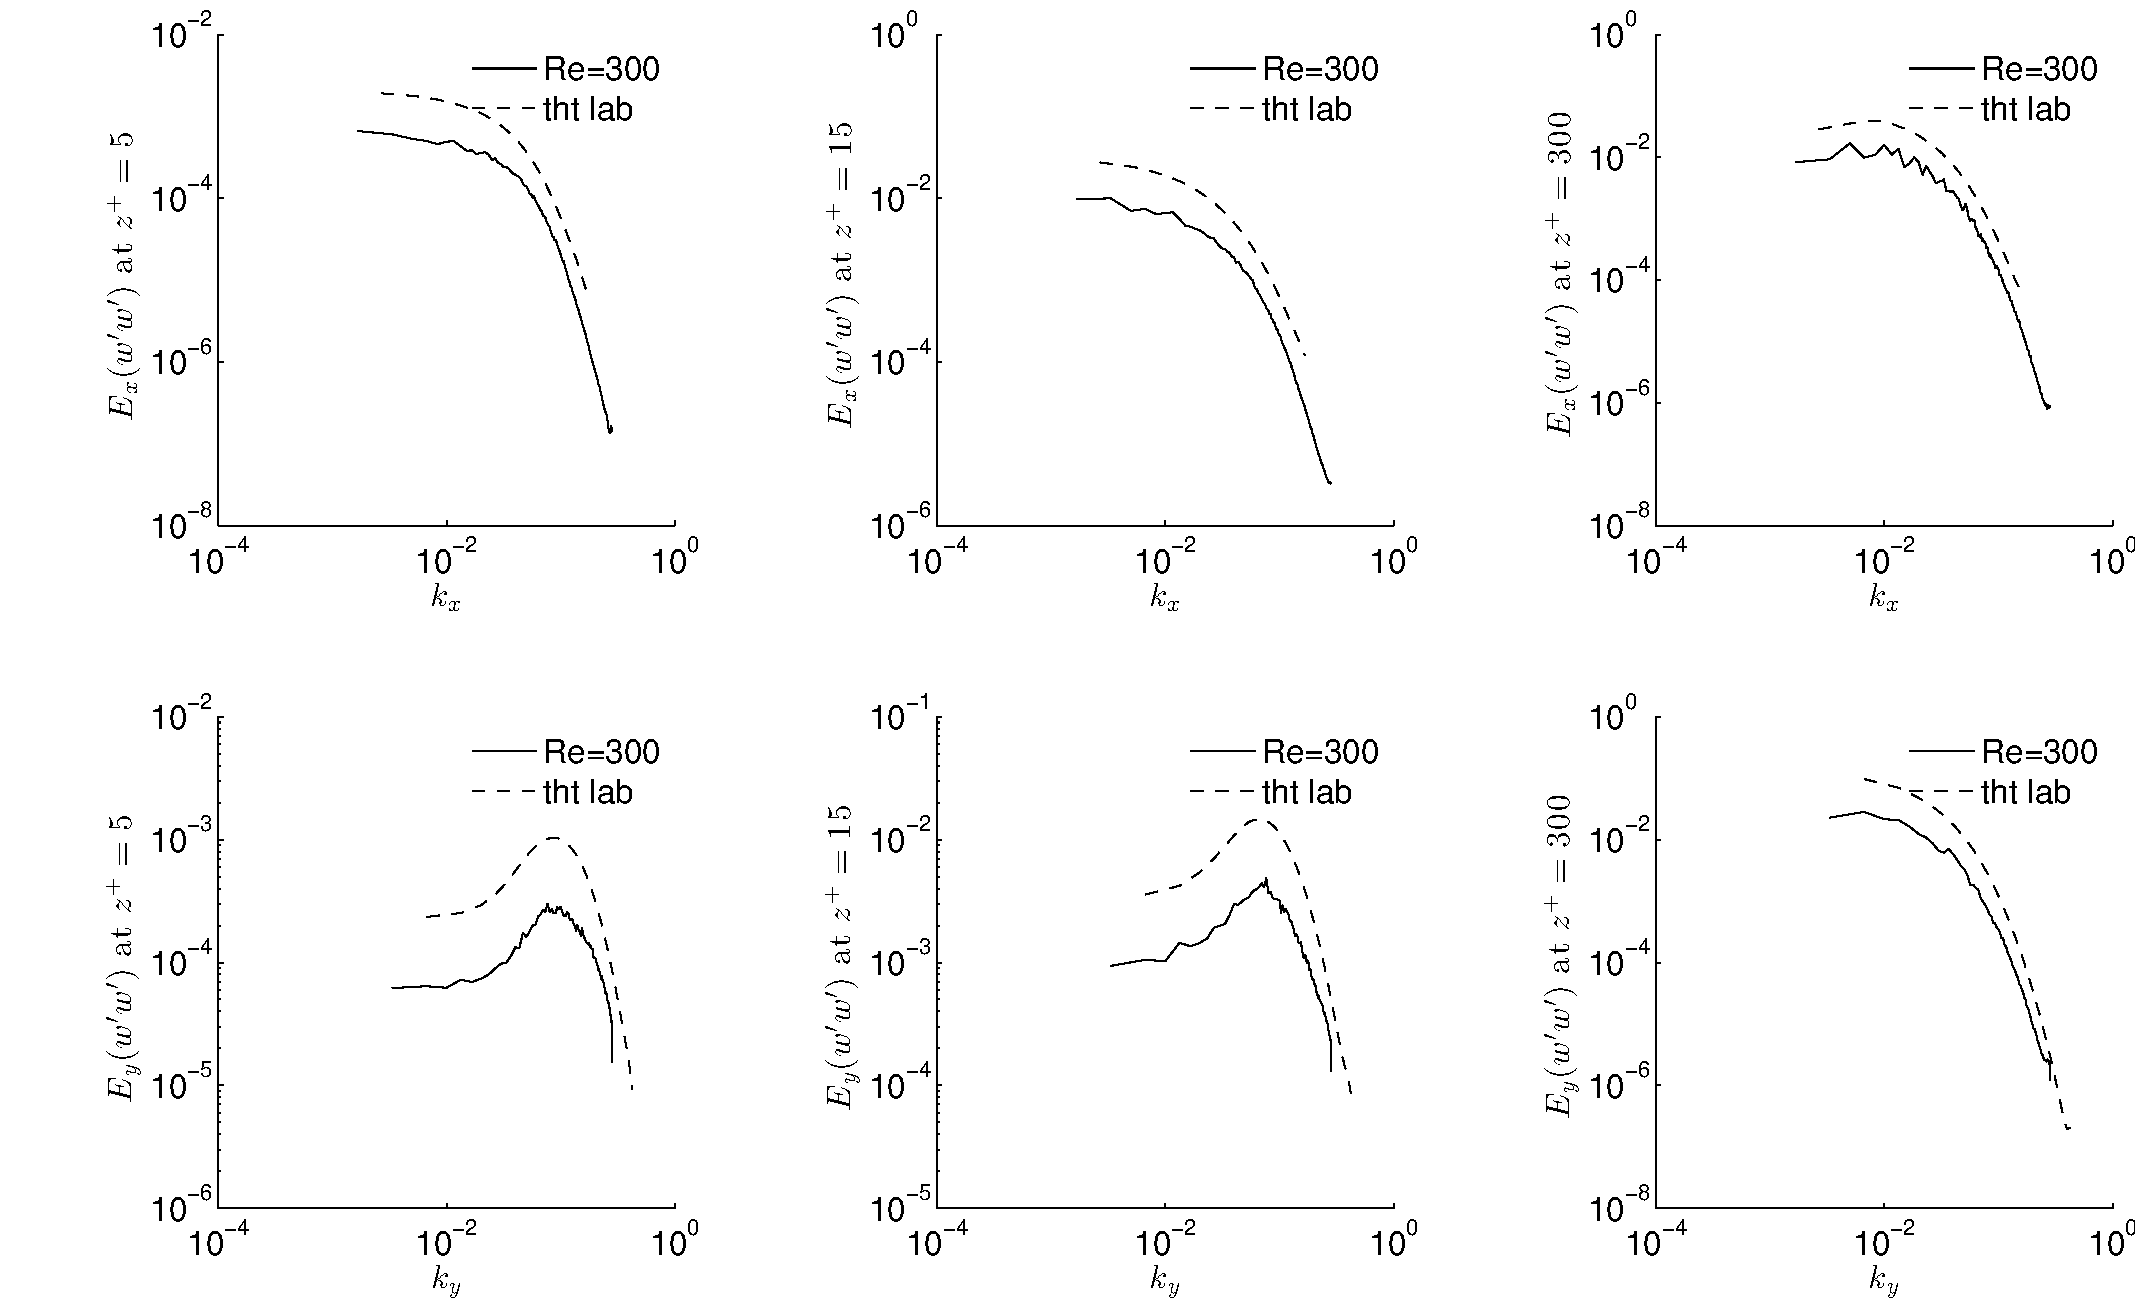
\includegraphics[width=\textwidth]{w_spectra}
\caption{$w'$ power spectra}
\end{sidewaysfigure}


\newpage
\section{Phase field validation}
The phase field was validated using the undamped analytical solution from \cite{Prosperetti81} for capillary waves at the interface between two superposed fluids (stable configuration). 
\begin{figure}[H]
\centering
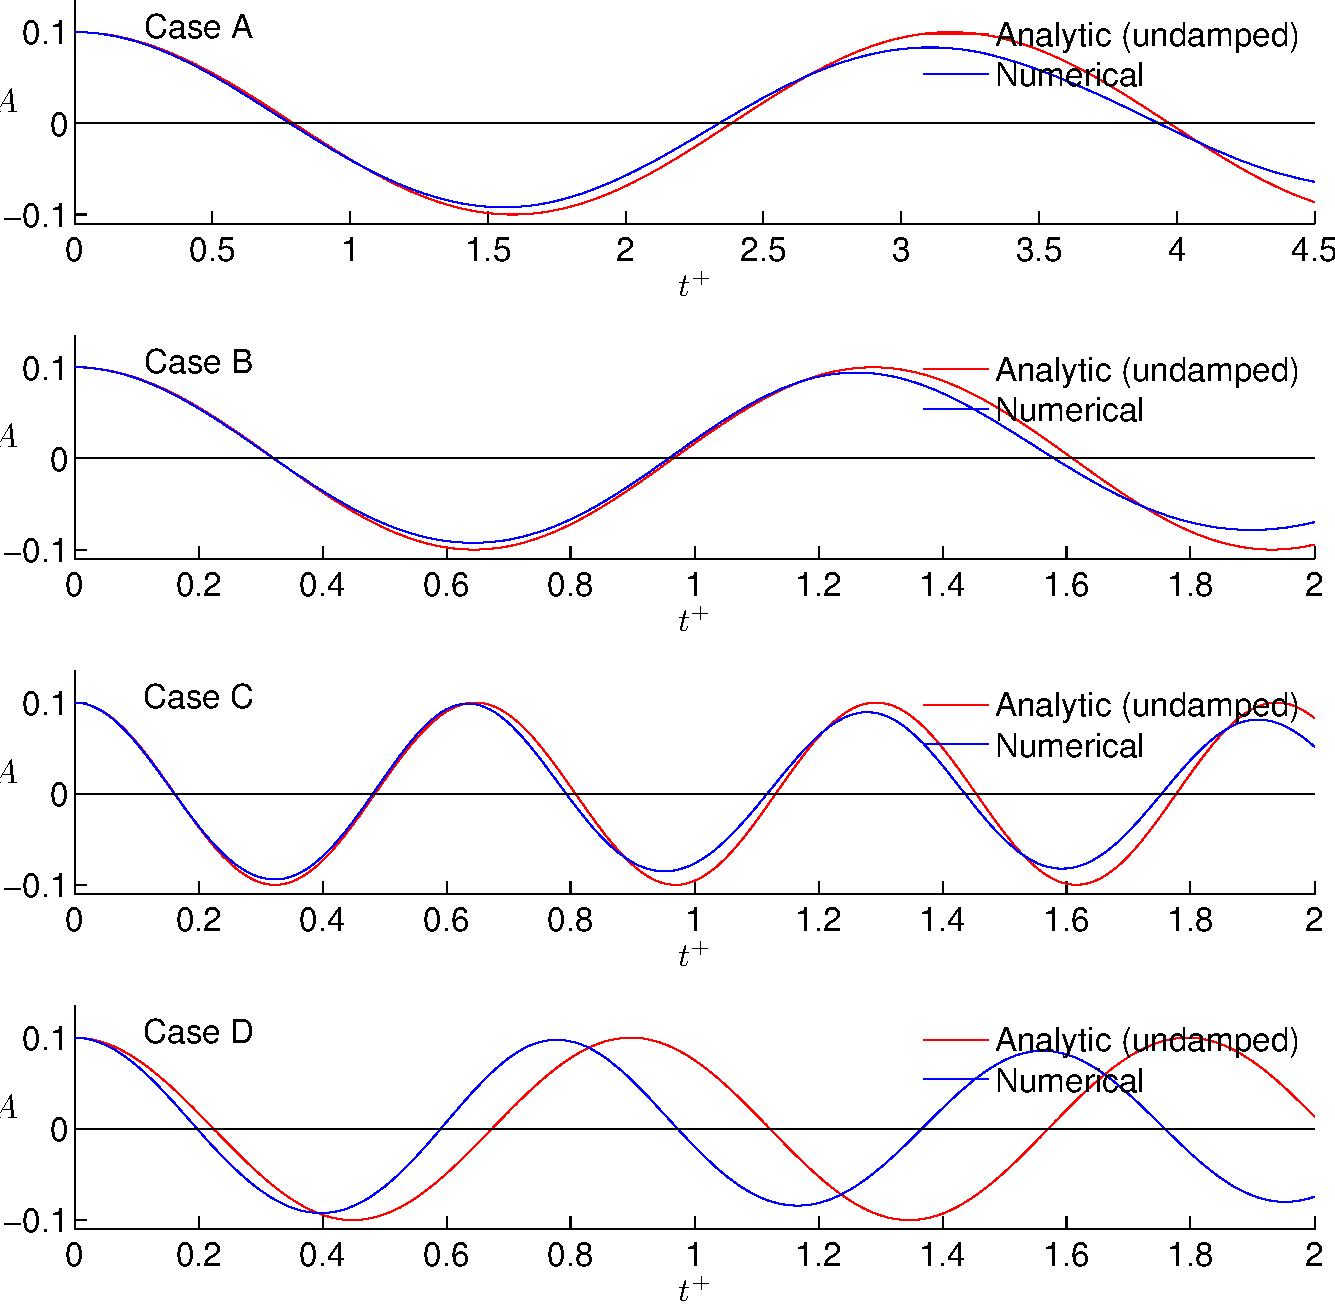
\includegraphics[width=\textwidth]{cap_waves}
\caption{Capillary waves, comparison of numerical solution (damped) with Prosperetti analytic solution (undamped). \textbf{Case A} : $\rho_R=0.9$, $\Fr=0.1$, $k_y=1$. \textbf{Case B} : $\rho_R=0.5$, $\Fr=0.1$, $k_y=1$. \textbf{Case C} : $\rho_R=0.5$, $\Fr=0.05$, $k_y=1$. \textbf{Case D} : $\rho_R=0.5$, $\Fr=0.1$, $k_y=2$.}
\end{figure}

\begin{table}[H]
\centering
\caption{Case run for phase field validation}
\begin{tabular}{l|c|c|c|c|c}
Case  & $\omega_0$ (analytic) & $\omega$ (numerical) & $\Delta \omega=\frac{\omega_0-\omega}{\omega_0}\cdot100$ [\%] & Density ratio & $\Fr$ \\[0.5ex]
\hline
Case A &1.976789 & 1.993080& -0.82  &0.9&0.1\\[0.5ex]
Case B &4.879132 &4.986655  & -2.20&0.5&0.1\\[0.5ex]
Case C & 9.721965& 9.933890&   -2.18&0.5&0.05\\[0.5ex]
Case D &7.001862 & 8.107336 &-15.79 &0.5& 0.1\\[0.5ex]
\end{tabular}
\end{table}



